\documentclass[a4paper,11pt,oneside]{book}
\usepackage{CS_report}
\usepackage{hyperref}
\usepackage{graphicx}
\usepackage{caption}

\begin{document}

\captionsetup[figure]{margin=1.5cm,font=small,name={Figure},labelsep=colon}
\frontmatter

\begin{titlepage}
    \begin{center}

        {\LARGE \textbf{CUNEF Universidad}}\\[0.4cm]
        {\large Double Degree in Business Administration and Computer Science}\\
        {\large Subject: Artificial Intelligence}\\[2cm]

        
\includegraphics[width=0.35\linewidth]{cunef.jpg}\\[2.5cm]

        {\Huge \textbf{Metro Simulation Project}}\\[0.4cm]
        {\Large Based on Discrete-Event Modeling}\\[1.2cm]

        \href{https://github.com/AlbertoCano4/subway-simulation}{\texttt{github.com/AlbertoCano4/subway-simulation}}\\[2cm]

        {\Large \textbf{Authors}}\\[0.3cm]
        {\large Alberto Cano\\
        Ignacio Fernández\\
        Gonzalo Ruiz}\\[2.5cm]

        \vfill
        {\large Madrid, April 4, 2025}

    \end{center}
\end{titlepage}

    \newpage
    \thispagestyle{empty}
    \chapter*{\centering \Large ¿Simulation or solution?}
    % -------------------------------------------------------------------


The northern region of Madrid has historically faced significant challenges regarding its integration into the city's metropolitan transport network. This lack of connectivity has not only impeded the daily mobility of residents but has also contributed to pronounced territorial inequalities, limiting access to economic opportunities, education, and essential services.
~\\[0,5cm]
Although initially conceived as a simulation, this project goes a step further. It emerges as a response to a real-world need: the poor connectivity of northern Madrid with the rest of the metropolitan transport network. This lack of infrastructure and accessibility in certain areas not only hinders the mobility of citizens but also deepens territorial inequalities within the city.
~\\[0,5cm]
Addressing the connectivity deficits in northern Madrid is imperative for fostering balanced urban development and social equity. By integrating advanced simulation techniques and artificial intelligence into transport planning, there exists a significant opportunity to design optimized network extensions. Such approaches can enhance route efficiency and improve the overall quality of life for residents, contributing to a more cohesive and accessible urban environment.
~\\[0,5cm]
Therefore, this work does not merely replicate the functioning of the Madrid Metro; it proposes a possible solution: an extension of the network that optimizes routes, improves efficiency, and considers the impact on users' quality of life. Through Artificial Intelligence techniques and simulation, the goal is not only to model the current system, but also to open a space for reflection and the design of more equitable and sustainable alternatives.
\begin{figure}
        \centering
        \vspace{-20 cm} 
        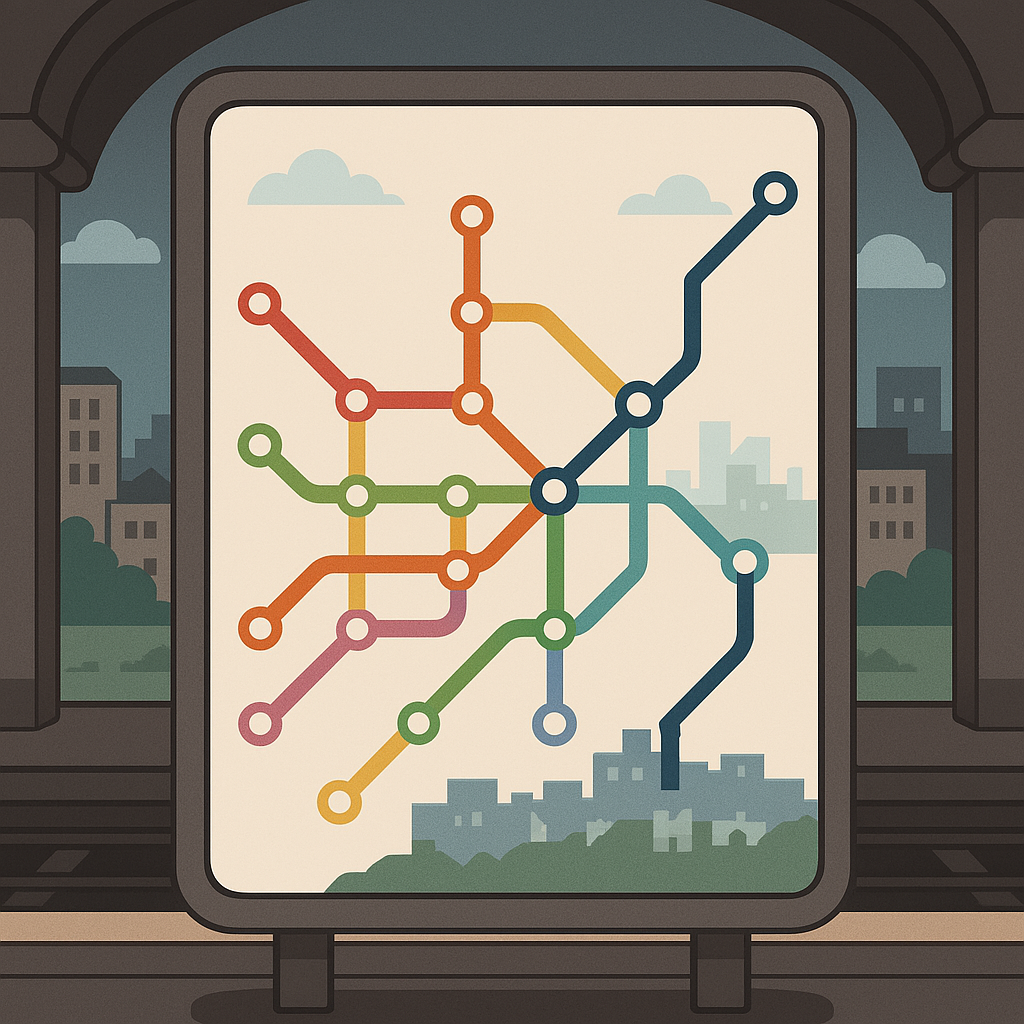
\includegraphics[width=0.49
        \linewidth]{image.png}
    \end{figure}





    % -------------------------------------------------------------------
    \newpage
    \thispagestyle{empty}
    \chapter*{\centering \Large Proyect Summary}


     We have developed a complete simulation of a metro system using discrete events in Python with the SimPy and NumPy libraries. The system models 10 stations connected by a circular line, with trains running in both directions (clockwise and counterclockwise). Passengers dynamically arrive at stations based on an arrival rate that varies with time of day, reflecting peak demand during rush hours. Trains are also generated according to the schedule, with more units active during high-demand periods, and are automatically withdrawn when no longer needed. Each relevant event, such as passenger arrivals, boardings, alightings, train arrivals, or train withdrawals, is recorded in an event-log.csv file along with its real-time timestamp (HH:MM). Additionally, the simulation uses a random seed to ensure reproducible results, allowing for consistent comparative analysis in a Jupyter notebook that extracts key operational metrics. 
    ~\\[0,5cm]
     Beyond the core functionality, the simulation incorporates additional features that bring it closer to real-world complexity. For instance, passenger arrival rates differ by station and fluctuate throughout the day, creating a more realistic representation of urban mobility patterns. Trains are programmed to follow specific directions and avoid collisions at stations, adding a layer of operational logic to the model. Furthermore, the system dynamically adapts to changing conditions: more trains are introduced during peak hours, and nonactive ones are retired to optimize energy and space usage. This dynamic behavior supports a better understanding of how transport systems can respond to varying demand throughout the day. 
     ~\\[0,5cm]
     We have also laid the foundation for future enhancements, including the integration of variable distances between stations, which would influence travel times and scheduling. This is crucial because in real metro systems, the stations are not equidistant, and the variation in travel time affects passenger flow and overall network efficiency. The code is structured to support scalability, allowing the addition of more complex scenarios such as line expansions, incident simulations, or advanced pathfinding algorithms. In general, this simulation serves as both a technical exploration and a decision support tool to design more adaptive and user-centered public transportation systems.\\
     


    \begin{figure}
        \centering
        \vspace{-10 cm} 
        \includegraphics[width=0.5\linewidth]{metro.png}
    \end{figure}

     
    
    
\chapter*{\center \Large  Code explanation }

This project simulates a metro system using SimPy, a discrete-event simulation library in Python, alongside NumPy for efficient data handling and random number generation. The system models a circular metro line with stations, trains, and passengers, where each component interacts dynamically according to time-dependent demand patterns. All major events (such as passenger arrivals, boardings, alightings, and train operations)are logged into a CSV file with precise timestamps. The number of active trains is automatically adjusted throughout the day based on predefined frequency schedules that adapt to peak and off-peak hours, ensuring realistic and scalable system behavior.


~\\[0,5cm]
\noindent\textbf{The main script:} central coordinator of the entire system. It initializes the SimPy environment, sets up time-handling utilities, and configures the logging of simulation events into a CSV file. In this file, relevant details like event type, station, time, and train identifiers are recorded. The script defines passenger arrival rates, generates stations along a metro line, and dynamically creates trains throughout the simulation. It adjusts train frequency according to simulated demand based on the time of day, ensuring the number of active trains reflects real-world peaks and valleys in usage.
~\\[0,5cm]
\noindent\textbf{The line module:} encapsulates the structure of the metro line itself. It manages the ordered list of stations, determines the next station a train should move to based on its direction, and calculates the number of stops between any two stations. It also includes a method to verify whether a train is heading in the correct direction to serve a passenger. This module acts as the network logic layer, ensuring passengers and trains follow consistent, rule-based movement through the circular metro system.

~\\[0,5cm]
\noindent\textbf{The Station module:} is responsible for simulating individual Station objects. Each station includes its name, current waiting passengers, and a rate at which new passengers are generated. This arrival rate changes dynamically depending on the time, simulating rush hours and off-peak periods. New passengers are assigned random destinations different from their current station, and all stations are connected to the metro line for consistent routing. This module helps simulate demand variability and station-level dynamics.

~\\[0,5cm]
\noindent\textbf{The Passenger module:} contains the Passenger class, which is a lightweight representation of users in the system. Each passenger holds an identifier and a destination station. The class includes a method for string formatting, useful for displaying or logging purposes. While simple, this module plays a crucial role in simulating realistic and individualized passenger movement throughout the network.


~\\[0,5cm]
\noindent\textbf{The Train module:} defines the logic for each Train object in the simulation. Each train has attributes such as its direction, capacity, current position, onboard passengers, and a reference to the overall line. Trains cycle through stations, allowing passengers to alight at their destination and boarding new ones when heading in the correct direction. The class includes mechanisms for avoiding station collisions and varying train travel time based on the time of day. It is also linked to the event logger, ensuring every action is recorded for later analysis.
~\\[1cm]
The main simulation function runs the train generation process, ensuring that the number of trains in circulation dynamically adjusts based on demand and the time of day. It also closes the event log file at the end of the simulation.
~\\[0,5cm]

In conclusion, the current version of the code is highly modular, with each file contributing a specific piece of the larger simulation. The design is scalable, easy to maintain, and well-prepared for integrating intelligent systems such as AI-based scheduling, passenger demand forecasting, or adaptive control strategies






   
    

\chapter*{\center \Large Jupyter Notebook }
The analisis. ipynb notebook is designed to examine the data generated during the simulation of the metro system, specifically those recorded in the eventlog.csv file. This file contains detailed information about every event occurring in the system, such as passenger arrivals at stations, train departures and arrivals, and boarding or alighting events. The analysis is performed using well-known Python data science libraries such as Pandas, Matplotlib, and Seaborn.
~\\[0,5cm]
\noindent\textbf{1. Boardings and Alightings by Station}
The analysis of boardings and alightings across stations reveals significant asymmetries in usage. Some stations act as strong departure hubs, likely located in residential or peripheral areas, while others dominate as arrival points, possibly situated near commercial, educational, or central zones. This directional flow highlights the existence of structural movement patterns in the simulated city model. Understanding these imbalances is essential for making targeted improvements in service frequency and infrastructure allocation.
~\\[0,5cm]
Moreover, these trends can inform planners about latent demand or underutilized parts of the network. Stations with few interactions might indicate areas with poor connectivity, insufficient accessibility, or low urban density, all of which could benefit from complementary policies. Enhancing last-mile connections, improving pedestrian access, or reinforcing intermodality with buses and bikes could help balance flows. As a simulation that mimics real urban inequality (like the poor connectivity in northern Madrid), this insight aligns with the broader social goal of reducing territorial disparities.
~\\[0,5cm]
\noindent\textbf{ 2. Passengers per Train   }
The distribution of boardings per train shows that certain units are heavily used while others remain underutilized. This suggests that some trains operate during high-demand windows or along particularly busy segments of the route. Conversely, trains with low boarding counts may correspond to off-peak hours, or operate in directions with less traffic flow. Identifying these load differences is crucial for adapting train deployment to actual usage patterns.
~\\[0,5cm]
From an operational standpoint, this imbalance could be addressed through dynamic train scheduling powered by predictive models. For instance, integrating AI to forecast demand could enable real-time activation or deactivation of trains based on expected ridership. Reducing idle capacity while maintaining service during critical times would improve energy efficiency and passenger experience. As your system already simulates dynamic train generation, this opens the door to future enhancements using reinforcement learning or fuzzy logic for even smarter scheduling.
~\\[1cm]
\noindent\textbf{3. Boardings per Hour }
The hourly boarding analysis confirms the presence of clearly defined rush hours, typically around 7–9 AM and 5–7 PM. These peaks align with expected commuter behaviors such as travel to and from work or school. The graph also highlights off-peak periods with minimal demand, where fewer trains may be necessary to maintain an efficient system. This temporal distribution validates the adaptive scheduling logic already implemented in your simulation.
~\\[0,5cm]
In a real-world context, this kind of temporal demand modeling is critical for resource optimization. Urban transport authorities could use such data to fine-tune service frequency and reduce operational costs during low-use hours. Moreover, these trends could be influenced by broader societal rhythms, like teleworking or school calendars, which an AI-enhanced system could learn to anticipate. Incorporating real historical data in future versions would allow your simulation to make even more accurate predictions and policy recommendations.
~\\[0,5cm]
\noindent\textbf{4. Top 10 Routes  }
The identification of the most frequently traveled routes offers deep insights into user preferences and network bottlenecks. These top 10 connections often represent direct links between major origin and destination pairs, acting as the backbone of the simulated metro line. A high concentration of passengers along these paths suggests their strategic importance, warranting special attention for upgrades or express service deployment. Monitoring their evolution over time can also reveal shifting patterns in urban mobility.
~\\[0,5cm]
From a planning perspective, prioritizing these routes could yield significant returns in user satisfaction and system performance. Increasing frequency, train capacity, or even offering dedicated lines during rush hours would help alleviate pressure and reduce travel times. Furthermore, these data points could serve as a validation metric when proposing new network extensions. In your case, given the project's intention to address connectivity gaps in northern Madrid, understanding which synthetic routes are most in demand can help shape realistic and equitable expansion strategies.
~\\[0,5cm]
\begin{itemize}
    \item Average Waiting Time per Station
This chart shows the average time passengers spend waiting at each station before boarding a train. It helps identify underserved stations and time slots with inefficient service.
\end{itemize}
\begin{itemize}
    \item Train Occupancy Over Time
This visualization tracks how full each train is throughout the day. It reveals usage patterns and highlights moments of overcrowding or underutilization.
\end{itemize}

\begin{itemize}
    \item Directional Flow Comparison
This chart compares passenger flow in clockwise vs. counterclockwise directions. It helps detect imbalances in network usage and supports direction-specific service adjustments.
\end{itemize}
   

    

  
    \begin{appendices}
        \chapter{Improvements for the next project}

\noindent\textbf{Areas for Improvement and Critical Assessment}
~\\[0,5cm]

While the current simulation successfully models a metro system using discrete-event principles and presents a solid foundational structure, future developments could significantly enhance its scalability, realism, and analytical depth—particularly through the integration of Artificial Intelligence (AI) and fuzzy logic techniques.
~\\[0,5cm]
Although the project is already organized into modular components , further abstraction would make the architecture more extensible. Defining higher-level classes, such as a MetroSystem controller or abstract entities like TransportUnit, would allow for easier implementation of features like multiple metro lines, interchange stations, or AI-driven routing and scheduling.
~\\[0,5cm]
Another technical improvement involves the modeling of travel times. Currently, all stations are treated as equidistant, which limits simulation realism. Introducing a matrix of variable distances or travel times between stations would allow for more accurate timing logic and could serve as a basis for algorithms that optimize train frequency based on real-time conditions.
~\\[0,5cm]
In terms of AI, future versions of the project could implement machine learning algorithms to dynamically adjust train frequency based on historical passenger data or predicted demand patterns. Supervised models could forecast peak times or station-level congestion, while reinforcement learning agents could be trained to manage scheduling decisions in real time to minimize waiting time and maximize system efficiency.
~\\[0,5cm]
Additionally, fuzzy logic could be incorporated to model more human-like or uncertain behaviors, such as passengers choosing between two stations or trains based on subjective criteria (e.g., "the train is too full", "I might wait for the next one"). This would bring more nuance and realism to passenger simulation, especially when decision-making cannot be captured by binary logic.
~\\[0,5cm]
Another key area for improvement is visualization. The project currently logs events to a CSV file for analysis, but lacks a visual interface. Adding a basic UI or data dashboard using tools like matplotlib, Plotly, or NetworkX would not only improve presentation quality but also help validate the model visually and make it more engaging for stakeholders.
~\\[0,5cm]
From a data perspective, the simulation currently uses idealized inputs. Integrating real-world datasets—such as passenger volumes, demographic trends, or transport usage statistics—would boost the system’s predictive value. Real station names, arrival behaviors, and urban constraints could be used to reflect the conditions of the Madrid Metro more accurately.
~\\[0,5cm]
Finally, the existing logging system could be extended to automatically analyze performance metrics, such as average waiting times, train occupancy, and bottlenecks. With AI and fuzzy logic integrated, the system could evolve into a smart decision-support platform for transport planners.
~\\[0,5cm]
In conclusion, this project provides a robust technical foundation and a clear social purpose. With the planned integration of AI, fuzzy logic, and real-world data, it has the potential to evolve into a sophisticated simulation and optimization tool for designing more intelligent, adaptable, and inclusive public transportation systems.
Lastly, from a user interaction perspective, the system lacks a visual interface that would aid in understanding the model and its results. A graphical interface, or at least a visual representation of the network and proposed routes, would have significantly increased the project's technical value and presentation quality.
~\\[0,5cm]
In summary, while this project offers a solid foundation, it also highlights critical limitations. These shortcomings must be addressed in future developments if simulation is to be a useful and interactive tool for urban transport planning.



        
    \end{appendices}
    
\end{document}
